\documentclass[10pt, letterpaper]{article}
\usepackage[utf8]{inputenc}
\usepackage[T1]{fontenc}
\usepackage{mathptmx} % Times New Roman (Formal & Compact)
\usepackage[margin=0.75in]{geometry} % Optimized margins
\usepackage{graphicx}
\usepackage{titlesec}
\usepackage{enumitem}
\usepackage{wrapfig}
\usepackage{xcolor}
\usepackage[hidelinks]{hyperref}
\usepackage{microtype} % Improved typography
\usepackage[spanish]{babel}

% --- FORMATO ---
\pagestyle{empty}
\setlength{\parindent}{0pt}
\setlength{\parskip}{0.5em}

% Estilo de secciones
\titleformat{\section}
    {\normalfont\large\bfseries\uppercase}
    {}{0em}{}[\titlerule]
\titlespacing*{\section}{0pt}{10pt}{5pt}

\begin{document}

% --- ENCABEZADO ---
\begin{center}
        {\Large \textbf{Cartograf\'ia musical emp\'irica: cuantificar la evoluci\'on estil\'istica}} \\
        \vspace{0.3em}
        \textbf{Victor Gurbani} $\cdot$ Suplemento de investigaci\'on $\cdot$ Solicitud oto\~no 2026
\end{center}

\vspace{-0.5em}

% --- CUERPO ---

\section*{1. Objetivo de investigaci\'on}
La musicolog\'ia suele apoyarse en descripciones subjetivas para categorizar el estilo: clasificar a Chopin como ``Rom\'antico'' o a Debussy como ``Impresionista'' a partir de una escucha cualitativa. Este proyecto busca sustituir la intuici\'on por medici\'on rigurosa. Mediante un flujo computacional de extremo a extremo, el objetivo fue cuantificar con precisi\'on los cambios arm\'onicos, mel\'odicos y r\'itmicos que definen la transici\'on desde el Per\'iodo de Pr\'actica Com\'un (Bach, Mozart) hacia finales del siglo XIX y comienzos del XX. En particular, quise comprobar si un algoritmo puede ``escuchar'' diferencias entre \`epocas sin sesgo humano.

\section*{2. Metodolog\'ia: el flujo computacional}
Se construy\'o un corpus equilibrado y seguro en cuanto a licencias de \textbf{144 partituras para piano solo} (36 de Bach, Mozart, Chopin y Debussy) a partir del archivo PDMX. Para procesar el conjunto, desarroll\'e un conjunto de herramientas en Python basadas en \texttt{music21}:

\begin{itemize}[leftmargin=*, noitemsep, topsep=0pt]
        \item \textbf{Extracci\'on de rasgos (36 m\'etricas):} el sistema calcula descriptores interpretables en tres dominios:
        \begin{itemize}[leftmargin=1.5em, nosep]
                \item \textit{Arm\'onico:} \textbf{densidad crom\'atica} (proporci\'on de tonos no diat\'onicos), \textbf{ratio de disonancia} (por ejemplo, notas de paso vs. apoyaturas) y distribuci\'on de calidades de acordes.
                \item \textit{Mel\'odico:} \textbf{entrop\'ia de alturas} (complejidad de la l\'inea) e \textbf{independencia de voces}.
                \item \textit{R\'itmico:} \textbf{ratio de sincopa} y \textbf{desviaci\'on est\'andar de duraciones} (una aproximaci\'on a rubato/fluid\'ez).
        \end{itemize}
        \item \textbf{Validaci\'on estad\'istica:} se aplicaron ANOVA de una v\'ia y pruebas post-hoc Tukey HSD ($p < 0.05$) para identificar qu\'e rasgos diferencian compositores, corrigiendo la tasa de descubrimientos falsos (FDR) para mantener el rigor.
\end{itemize}

\section*{3. Resultados clave}
% --- FIGURA ENVUELTA (Prueba de validaci\'on) ---
\begin{wrapfigure}{r}{0.5\textwidth}
        \vspace{-18pt}
        \centering
        \href{https://victor-gurbani.github.io/JuFo2026/figures/highlights/ravel_string_quartet_pca_cloud.html}{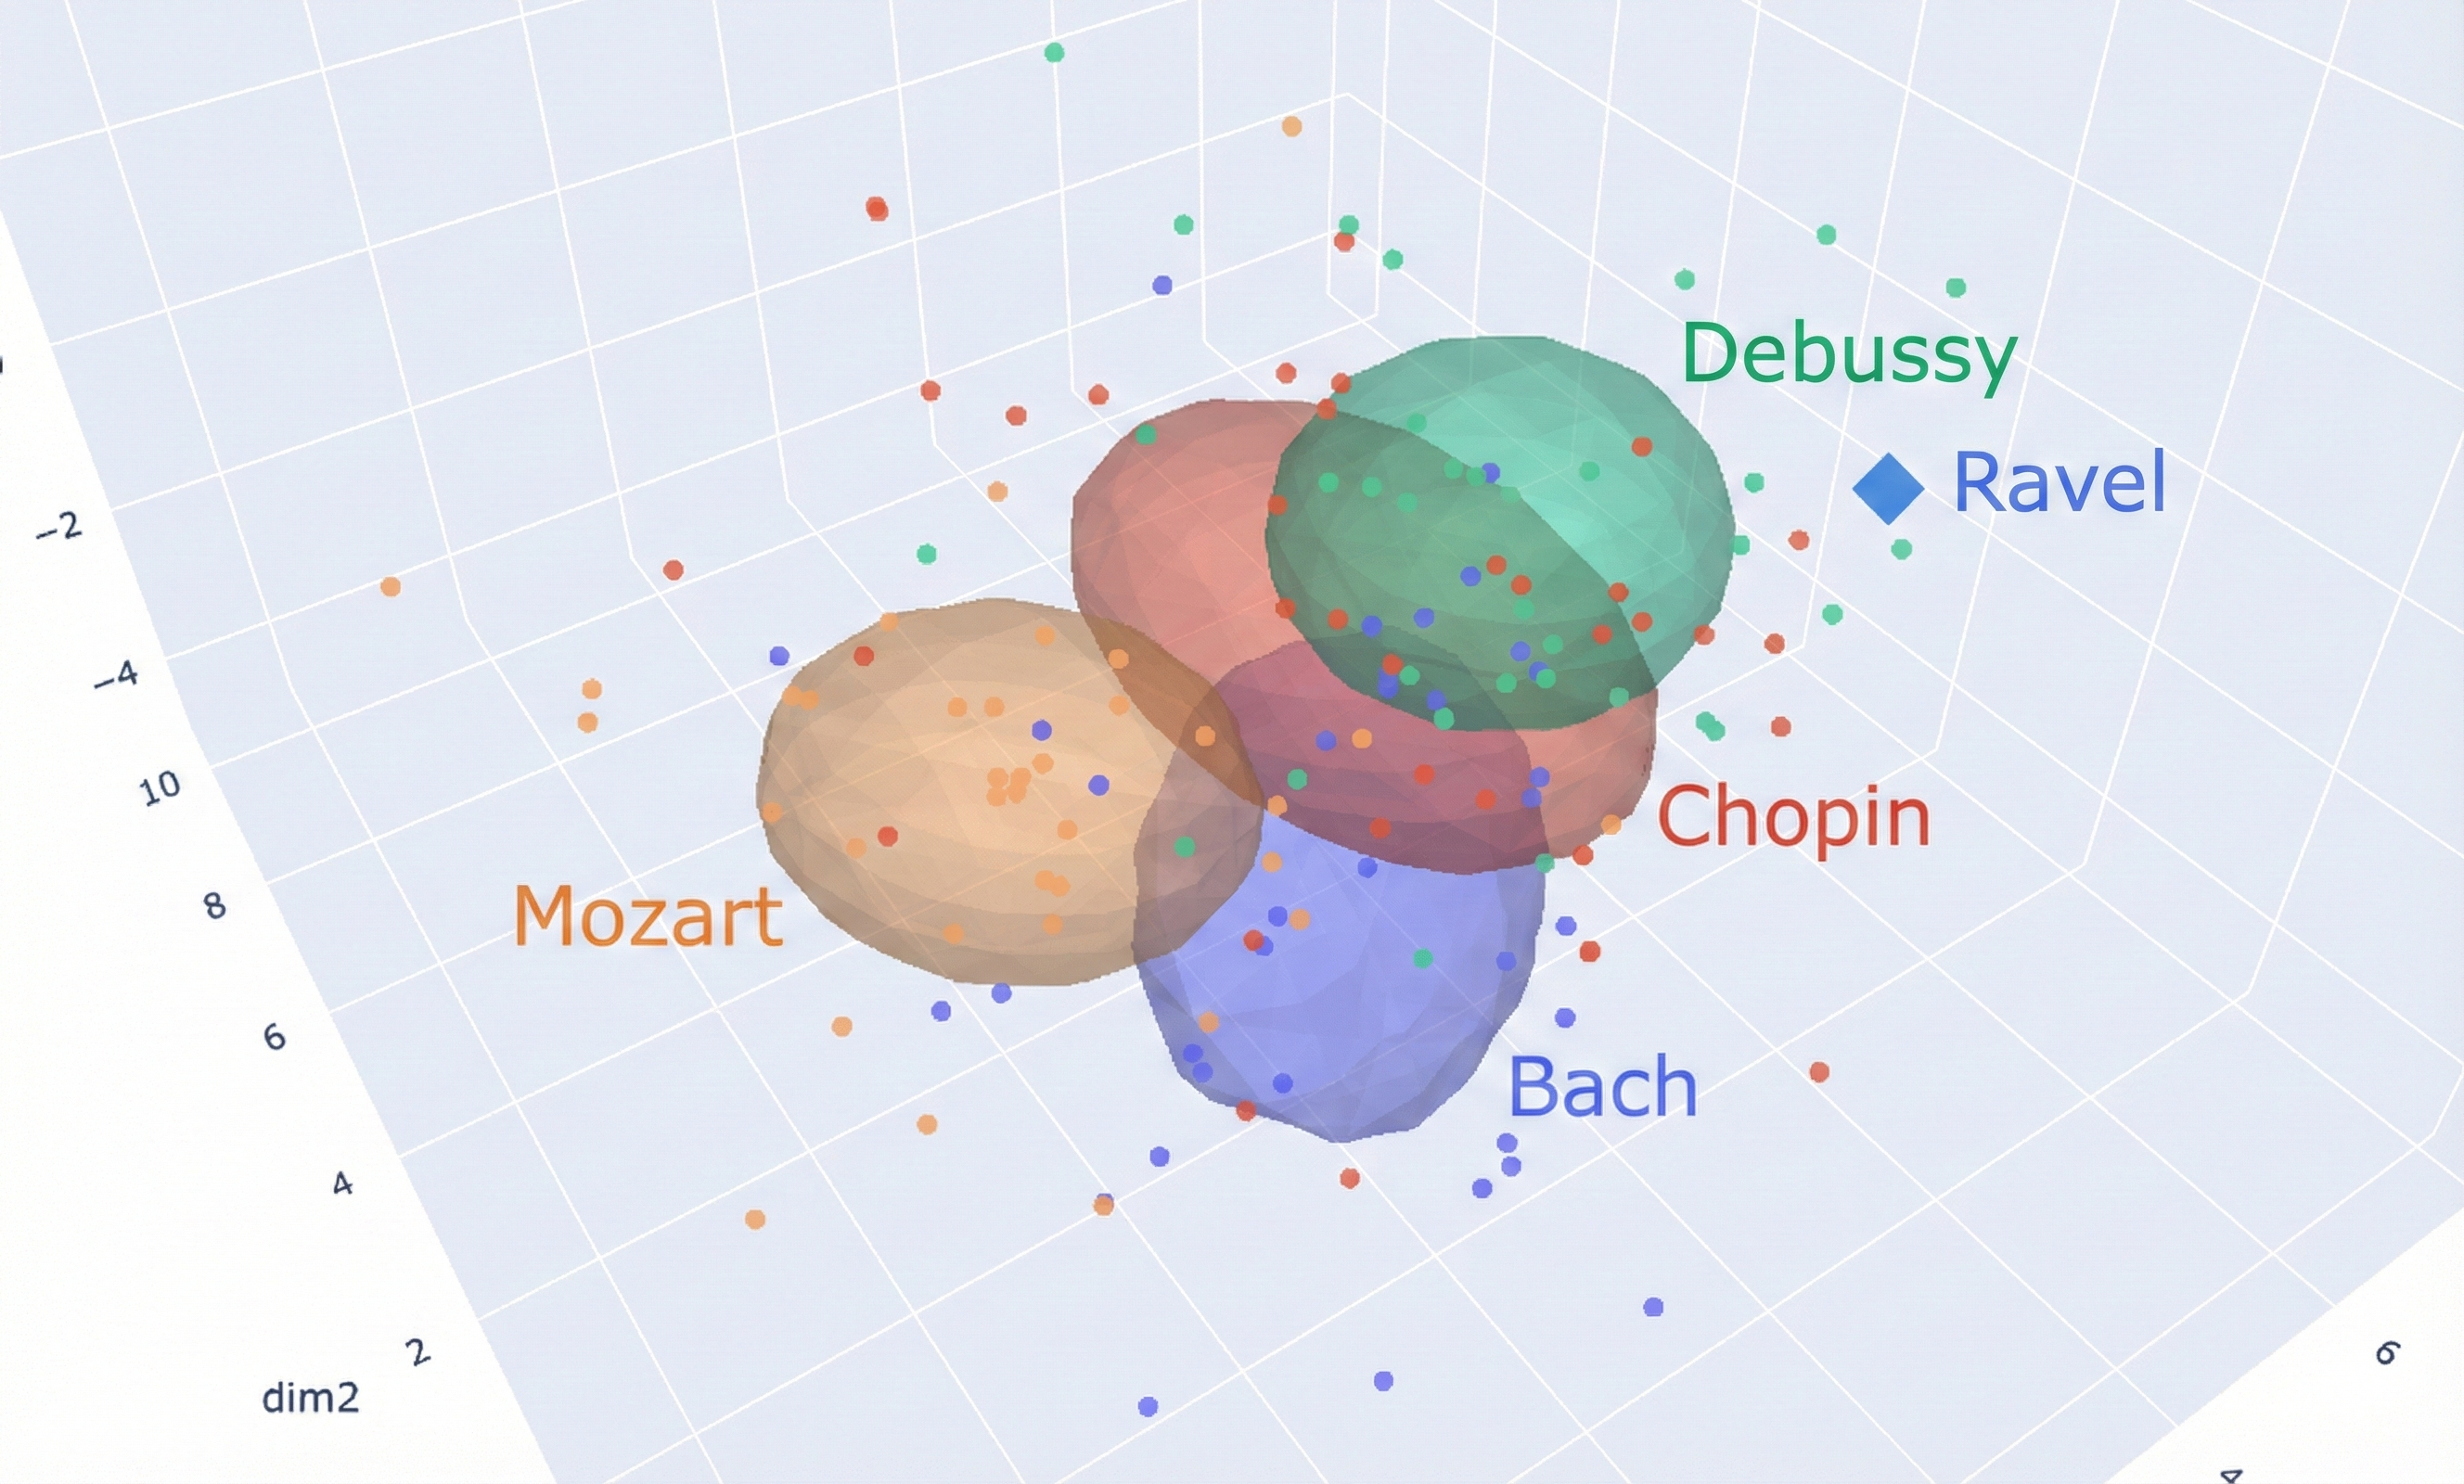
\includegraphics[width=0.48\textwidth]{ravelhighlight_cropped.png}}
        \vspace{-10pt}
        \caption{\small \textit{\textbf{Figura 1: proyecci\'on PCA del espacio estil\'istico.} El marcador en forma de rombo ($\diamond$) representa el caso de prueba no visto: el Cuarteto de cuerda en Fa de Ravel. El modelo lo proyecta m\'as all\'a del grupo de Debussy, cuantificando la progresi\'on hacia el post-impresionismo. (\href{https://victor-gurbani.github.io/JuFo2026/figures/highlights/ravel_string_quartet_pca_cloud.html}{\textcolor{blue}{Abrir}}).}}
        \vspace{-10pt}
\end{wrapfigure}
El an\'alisis estad\'istico confirm\'o que \textbf{29 de las 36 m\'etricas} distinguen de forma significativa. El An\'alisis de Componentes Principales (PCA) aporta una narrativa matem\'atica clara, donde las nubes de color representan el corpus de entrenamiento:

\begin{itemize}[leftmargin=*, noitemsep, topsep=0pt]
        \item \textbf{El ``puente Chopin'':} Chopin ocupa un espacio transicional. Su estructura de fraseo (PC2) se alinea con la disciplina de Bach/Mozart, pero su densidad crom\'atica y complejidad r\'itmica (PC1/PC3) lo acercan a Debussy. Act\'ua como el v\'inculo matem\'atico entre claridad cl\'asica y color impresionista.
        \item \textbf{Diferenciar a Debussy:} Debussy aparece estad\'isticamente aislado. Sus partituras muestran las tasas de disonancia m\'as altas ($p < 1.3 \times 10^{-10}$ frente a Bach) y una entrop\'ia r\'itmica elevada, cuantificando el efecto de ``difuminado'' asociado al impresionismo.
\end{itemize}

\section*{4. Validaci\'on del modelo: la ``prueba Ravel''}
Para comprobar el poder predictivo del modelo, se introdujo una obra no vista fuera del corpus de entrenamiento: \textbf{el \textit{Cuarteto de cuerda en Fa mayor} de Maurice Ravel}.

Como se observa en la \textbf{Figura 1}, el modelo ubica a Ravel en la regi\'on estil\'istica correcta sin etiquetado manual. En particular, Ravel aparece \textit{m\'as} avanzado en el eje del componente principal que Debussy. Esto respalda cuantitativamente la teor\'ia musicol\'ogica de que Ravel expandi\'o las texturas impresionistas hacia estructuras a\'un m\'as complejas y fluidas. El resultado sugiere que las 36 m\'etricas no solo describen el pasado, sino que tambi\'en capturan direcciones de evoluci\'on estil\'istica.

\section*{5. Importancia}
Este trabajo conecta arte y ciencia de datos, ofreciendo un marco reproducible para la \textit{musicolog\'ia computacional}. Al tratar partituras como datos, las teor\'ias hist\'oricas pueden contrastarse con evidencia emp\'irica, mostrando que la ``sensaci\'on'' de una \`epoca musical se sustenta en cambios estructurales cuantificables.

\end{document}
